\section{Introduction}

Artificial Intelligence (AI) is a field of computer science focused on developing hardware and software systems capable of performing tasks that typically require human intelligence. 
These systems can autonomously pursue specific goals by making decisions that were traditionally made by humans.

A key distinction in AI-driven systems lies between smart objects and connected objects.
While connected objects primarily send and receive data from the cloud, smart objects analyze data locally, enabling faster decision-making and reducing reliance on constant connectivity.

The definition of AI evolves rapidly, to the point that what was considered AI a decade ago may differ significantly from today's understanding.

AI hardware and software can be categorized similarly to traditional computing environments but are specifically designed to handle AI workloads. 
In this context, the development environment is often referred to as a framework, platform, or tool, rather than just a conventional programming environment.
\begin{figure}[H]
    \centering
    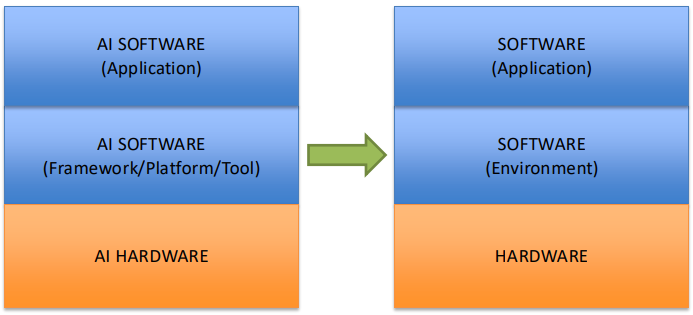
\includegraphics[width=0.5\linewidth]{images/eeai1.png}
    \caption{Artificial Intelligence stack}
\end{figure}
The AI stack consists of three main layers:
\begin{itemize}
    \item \textit{Application}: AI-powered applications running within an IT system.
    \item \textit{Framework, platform and tools}: programs and libraries that manage physical resources and provide the necessary tools for building AI applications.
    \item \textit{Hardware}: the infrastructure supporting AI computation, including data centers, edge computing devices, IoT systems, and specialized processors.
\end{itemize}